\chapter{Overview of Method and Tools Used}\label{ch:method}
%\section{Overview of the tool}
The aim of this thesis is to provide sound designers with an easy-to-use tool which enriches video games with procedural and physics-based audio instead of having to use prerecorded sounds. The tool enables to control contact sounds (impact, rolling and scratching) produced by vibrating objects through high level parameters that characterize the objects (size, material and surface roughness). The challenge is to offer realistic real-time and event-based sounds without high CPU usage.

\Todo{replace figure  with a better one}
\begin{figure}[H]
  \centering
    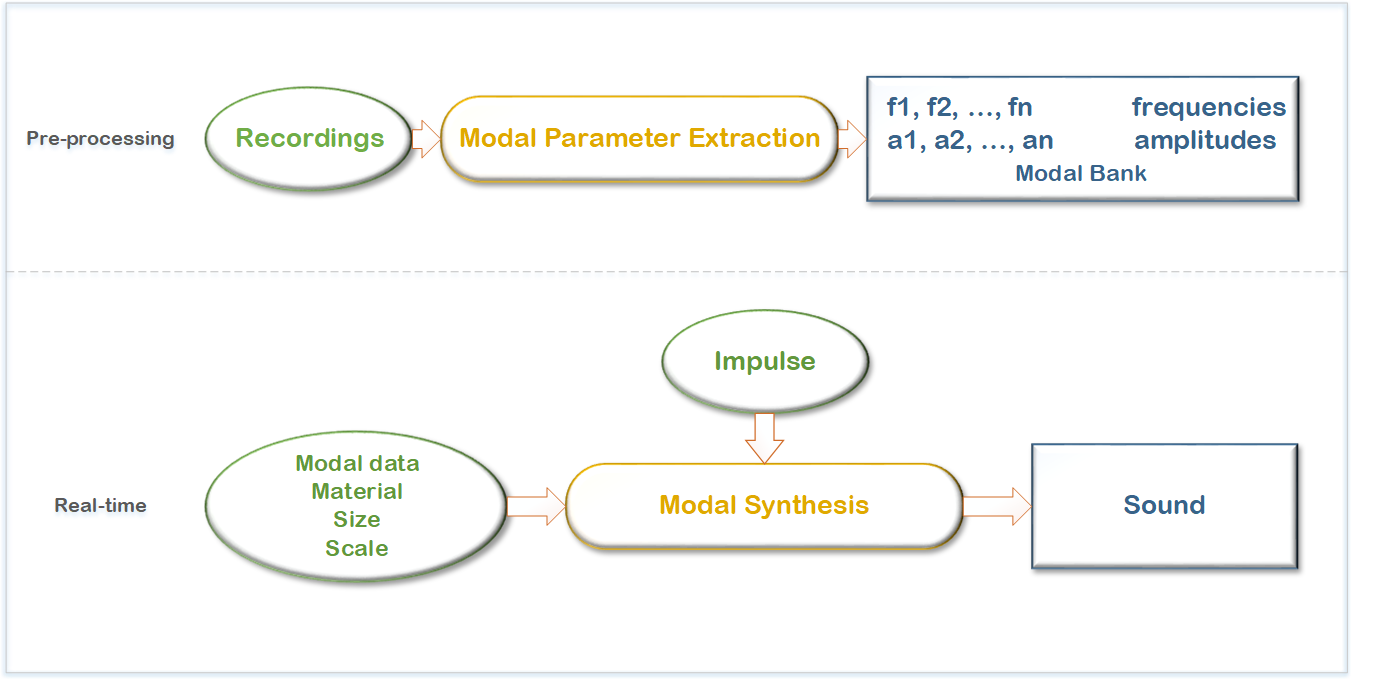
\includegraphics[width=\textwidth]{overview.png}
      \caption{Tool overview.}
      \label{fig:synth_proc}
\end{figure}

To create this tool, the procedure described in figure \ref{fig:synth_proc} was followed. To extract the modal parameters of vibrating objects the ``Example-guided'' method described in \ref{sec:exampleguided} was used due to its better integration within the audio pipeline as opposed to the rest of techniques presented in \ref{sec:modal_extraction}. The first step was to find several everyday objects that were made of different materials (plastic, wood, ceramic, glass and metal). This is because a priority in this thesis is the synthesis of sounds based on material properties. To obtain sound variations along the object's surface (see second method in \ref{sec:sound_variation}) the chosen objects were divided into areas that produced similar sounds when struck (e.g. bottle neck, rim of glass, etc). Between two and six sounds were recorded depending on the object. An example is presented in the following section for illustration \ref{sec:recordings}.

The recordings were then used to extract the data needed for the sound synthesis with the ChucK programming language. Some involved \gls{DSP} algorithms that employ the \gls{FFT} are used to capture the modal frequencies and gains specific of the object and which are present in the supplied audio clips. This process is explained in more depth in section \ref{sec:chuck}. 

As far as the modal synthesis of impact sounds is concerned, the two methods shown in \ref{sec:modal_synth} have been implemented into Pure Data patches \ref{sec:impact_synth} to evaluate differences between the output sounds. Scratching and rolling sounds (see \ref{sec:scratching_synth} and \ref{sec:rolling_synth} respectively) also make use of the filter-based method.

 At the same time, we made a 3D model of every object we used. We combined the 3D models with their corresponding data and the synthesis patches inside Unity\textsuperscript{\textregistered} software \cite{bib:unity}. At this point, the frequencies and amplitudes corresponding to the point of collision are assigned to the patch. The sound is then sent to the audio DSP chain and is played back. 

\section{Recordings}
The first step of this tool creation is to obtain the necessary data for audio synthesis. Thus, we performed recordings of the sound produced of the object when being hit in several areas. The signal of those recordings was used to extract the modal frequencies and their peaks. 

Since we only used simple shape everyday objects, we could easily assume that nearby points produce almost the same sound and thus separate the object into ``sound areas'' instead of calculating different modal matrices for each vertex. Unofficial tests proved that this accuracy-computational complexity trade-off was acceptable. A sample object and its division in areas is shown in figure \ref{fig:pot_sep}.

\begin{figure}[H]
  \centering
    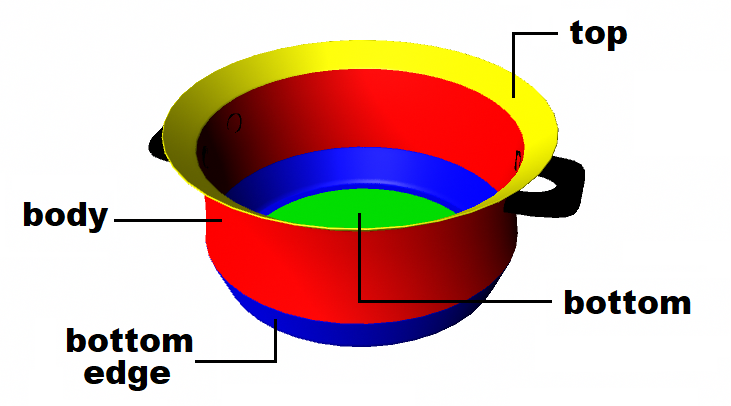
\includegraphics[width=0.6\textwidth]{potseparated.png}
      \caption{Division of an object into areas with similar sound.}
      \label{fig:pot_sep}
\end{figure} 

The procedure of the recordings will be explained in detail in section \ref{sec:recordings}.

The reason why we chose to extract the modal data from recordings instead of using the FEM method as in \cite{director2001synthesizing} or \cite{o2002synthesizing} or using spring-mass systems as in \cite{raghuvanshi2006interactive} lays in simplicity. More specifically, recordings of impact sounds is much easier for our target users to perform, if they want to extend our tool, than having to use complex calculations or software.

\section{3D models}
To achieve realistic sounds, we have to correspond the impact recordings of the real objects with same size 3D models of them. Hence, we measured the dimensions and weight of the eleven objects and used those data to model the objects. In table \ref{tab:dim_weig} the maximum dimensions and the weight of the objects are displayed. To create the 3D models of the objects we used \textbf{Maya Autodesk} software \cite{bib:maya} and exported them as FBX\textsuperscript\textregistered\ files \cite{bib:fbx} which is a format recognizable by Unity\textsuperscript{\textregistered}.

\begin{table}[H]
	\centering
    \begin{tabular}{ l c r c}
    \toprule
    \textbf{Name} & \textbf{Dimensions(cm)} & \textbf{Weight(g)} & \textbf{Picture} \\
    \toprule 
    Cooking pot & $21.5L\times 21.5W\times 10.8H$ & 680 & 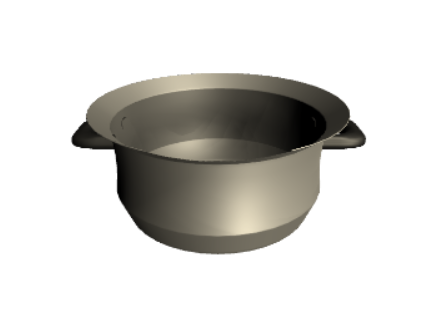
\includegraphics[scale=0.1]{3DmodelsPics/cp.PNG} \\ 
    Cup & $7.5L\times 7.5W\times 6H$ & 125 & 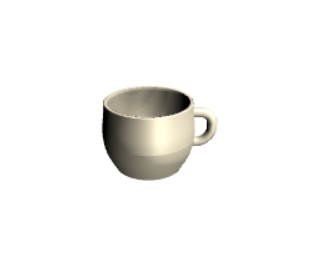
\includegraphics[scale=0.1]{3DmodelsPics/cup.PNG} \\ 
    Cutting board & $41.5L\times 26.5W\times 4.5H$ & 2200 & 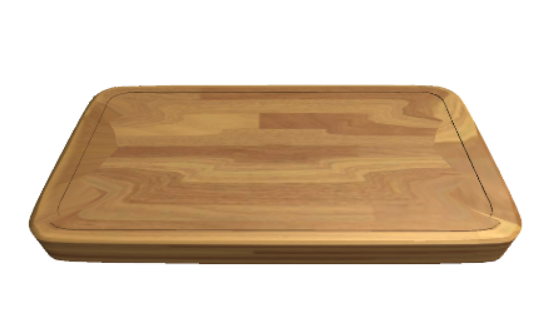
\includegraphics[scale=0.1]{3DmodelsPics/cb.PNG} \\ 
    Jug & $14L\times 10W\times 21.5H$ & 150 & 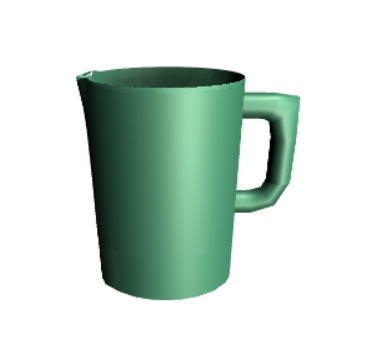
\includegraphics[scale=0.1]{3DmodelsPics/jug.PNG} \\ 
    Mortar & $11L\times 11W\times 19H$ & 850 & 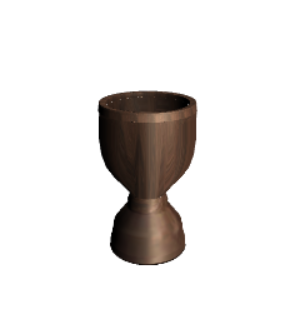
\includegraphics[scale=0.1]{3DmodelsPics/mortar.PNG} \\
    Bowl & $20L\times 20W\times 10.5H$ & 100 & 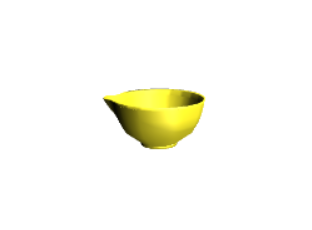
\includegraphics[scale=0.1]{3DmodelsPics/bowl.PNG} \\
    Plate & $25.5L\times 25.5W\times 2.5H$ & 700 & 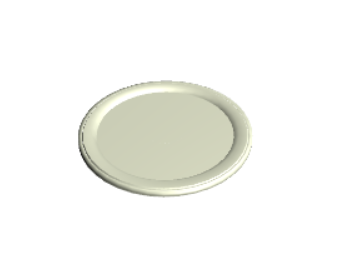
\includegraphics[scale=0.1]{3DmodelsPics/plate.PNG} \\
    Rolling pin & $43L\times 7W\times 7H$ & 700 & 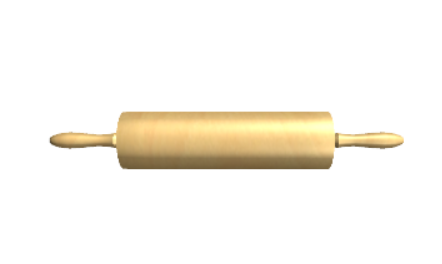
\includegraphics[scale=0.1]{3DmodelsPics/rp.PNG} \\
    Wine bottle & $7L\times 7W\times 29H$ & 400 & 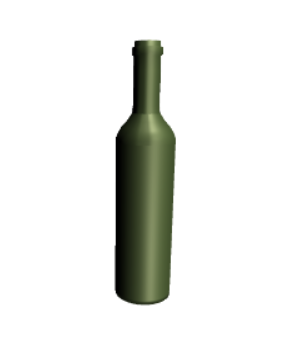
\includegraphics[scale=0.1]{3DmodelsPics/bottle.PNG} \\
    Wine glass & $8L\times 8W\times 18H$ & 120 & 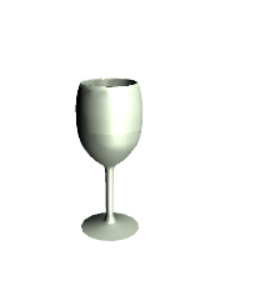
\includegraphics[scale=0.1]{3DmodelsPics/glass.PNG} \\
    Wok & $35L\times 35W\times 9.5H$ & 1225 & 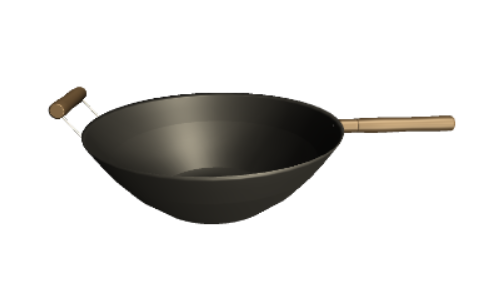
\includegraphics[scale=0.1]{3DmodelsPics/wok.PNG} \\
    \bottomrule
    \end{tabular}
    \caption{Maximun dimensions and weight of the eleven objects.}
    \label{tab:dim_weig}
\end{table}

%     \begin{minipage}{.45\textwidth}
%      \begin{itemize}
%        \item Cooking Pot
%		\item Cup
%		\item Cutting Board
%		\item Jug
%		\item Mortar
%		\item Bowl
%		\item Plate
%		\item Rolling Pin
%		\item Wine Bottle
%		\item Wine Glass
%		\item Wok
%     \end{itemize}
%  \end{minipage}
%    \begin{minipage}{.45\textwidth}
%    	\hspace{-3cm}
%    		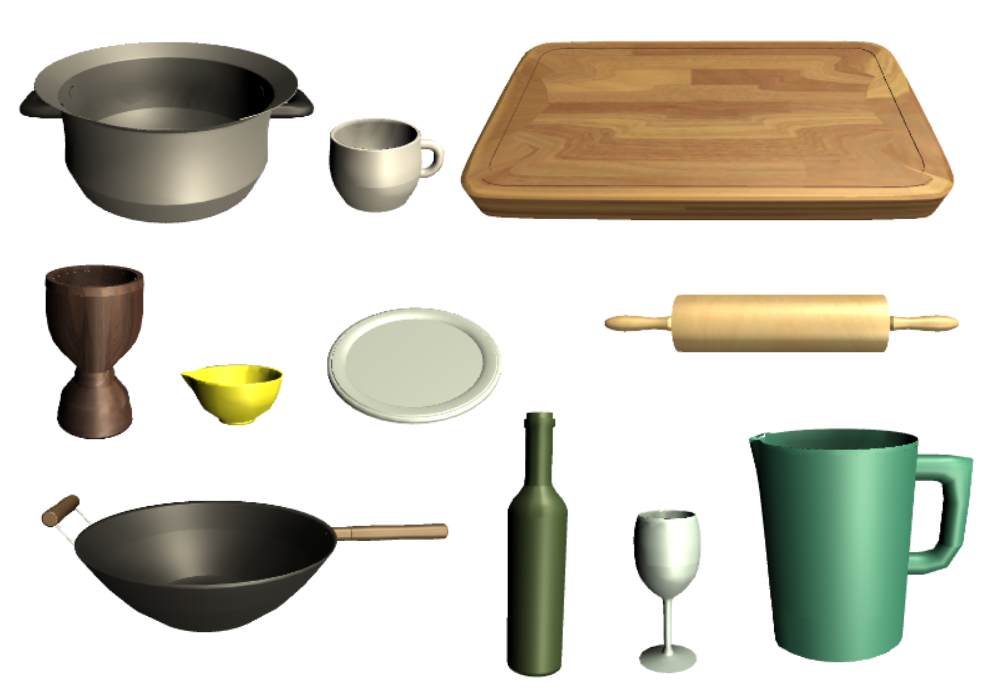
\includegraphics[scale=0.4]{3DmodelsPics/3dmodels.png}
%     		 \label{fig:3d_all}
%    \end{minipage}

\section{Modal data extraction}\label{sec:chuck}
\textbf{Chuck} language is a music programming language, made for ``real-time sound synthesis and music creation'' as mentioned in their website \cite{bib:chuck}. It's biggest advantage is the way it manipulates time. More specifically, the user specifies how long a sound will last, independent of other sounds that may play at the same time.

We used the ChucK language at the starting point of our thesis to identify and extract the peaks of the recorded audio files. The algorithm used in this part of the thesis is made by Perry Cook for the course \textbf{``Physics-Based Sound Synthesis for Games and Interactive Systems''} held by \textit{Perry Cook} and \textit{Julius O. Smith} at \textbf{Kadenze Academy} \cite{bib:physicsbasedcourse}.

From a modal analysis one can find out that each object vibrates in a very high number of modes. Although, most of them are inaudible and do not contribute to the sound model. It is, therefore, desirable to preserve CPU cycles by reducing the number of calculated modes. Based on the recommendations of the author Perry Cook, we chose ten as the sufficient amount of modes for the analysis/synthesis.  Afterwards, the algorithm having taken a recording as input, computes its histogram and identifies its peaks. The frequencies where peaks occur are the modal frequencies candidates. Depending on the numbers of peaks we chose, the algorithm outputs the strongest peaks. Finally, the algorithm finds the maximum value of the signal on each peak, calculating the corresponding amplitude of each mode.

ChucK language was chosen, because of its build-in functions to manipulate sound like \textit{Fast Fourier Transform (FFT)} of input audio samples and windows functions \cite{bib:chuck_doc}. Another option to extract the peaks of the sound waves could be to use python programming language on audio files, but this would request to program a number of functions or include a number of libraries that perform actions like file input/output, FFT and more. 

\Todo{should we explain why we used FFT?} 
 
\section{Modal synthesis patches}
\textbf{Pure Data (Pd)} is another music programming language. It is open source and the main difference from ChucK language is that Pd is a visual or ``patcher'' programming language, using objects instead of code, linked together to form a sequence \cite{bib:pd}. We chose to use this software as our synthesis engine mainly because of the ability to compile the patches into C\# code, as explained below in section \ref{sec:heavy}. Another important reason for choosing it is the possibility of real-time parameter manipulation and easy testing during implementation period.

All synthesized sounds (impact, rolling and scratching) are being synthesized under one main pd patch. However, two different patches have been developed, one for each of the two examined methods. Since the audio synthesis patch takes the modal data as input, every object can use the same patch. The synthesis patches will be described in detail in section \ref{sec:synthesis_implem}.

%For optimization reasons, we lowered the number of modes down to 10 instead of 20 that we initially had, since the extra 10 did not add any useful information to the output sound. In addition, we clipped the range of frequencies to the human audible range of 20Hz to 20KHz. 

\Todo{develop more?}

\section{Heavy Compiler}\label{sec:heavy}
\textbf{Heavy} is a compiler that generates audio plugins from Pd patches in interactive sound and music applications \cite{bib:heavy}. In this thesis we used it to compile Pd patches into Unity\textsuperscript{\textregistered} audio plugins. Heavy's interface is their website where users upload patches and then are able to download the corresponding plugins and put them into their applications. The plugins we used consist of DLL files and a C\# (Unity\textsuperscript{\textregistered} code) script that allows communication of the plugins with the rest of the scripts and also enables the sound card to play audio.

Through the generated C\# script, we are able to send float values to the audio plugins - which are the compiled Pd patches - as inputs to generate the appropriate sound. Those floats are the frequencies and their corresponding amplitudes, the quality factor (Q-factor) of the band-pass filters, the impact force of the collision, the roughness of the object, the multiplier of the size of the object, the velocity of the object and the rolling and scratching duration times. A difficulty we encountered by using this compiler was the inability of sending a whole array or list of floats. Thus, we had to send every frequency and every amplitude individually, creating a float parameter for each.
 
\subsection{Why not OSC?}
The most popular way to communicate between Unity\textsuperscript{\textregistered} and Pure Data is the Open Sound Control (OSC) protocol. The reason why we did not use it is because it requires establishing a connection between two software programs and send data between them. On the other hand, Heavy makes everything work inside Unity\textsuperscript{\textregistered} and it is as simple as passing floats between scripts. 

\section{Unity\textsuperscript{\textregistered}}
\textbf{Unity\textsuperscript{\textregistered}} is a game engine software. This is where all previous work is combined together and outputs the final product. For the purpose of this thesis, several demonstration scenes are made inside Unity\textsuperscript{\textregistered} where objects are struck in several points and produce different sounds. 

The first part of the Unity\textsuperscript{\textregistered} implementation is the assignment of modal data to every different area of the object. This is done in linear time ($O(n)$ for $n$ modes). The whole procedure of assigning the appropriate data includes the identification of the area of the object that collided, filling the arrays with the corresponding data and set the parameters of the plugins. Afterwards, the type of collision is identified and a number of other parameters are calculated and sent to the plugins, like the impact force and the duration of the collision.

Audio in Unity\textsuperscript{\textregistered} is enabled using the \textit{OnAudioFilterRead()} function. This function is running in the audio thread, which is a different one from the main thread. Its job is to send the audio buffer to the sound card and is called every $\sim 20$ms, so it does not require a function call from the programmer \cite{bib:unity_doc}.

\section{Microsoft Hololens Emulator}
\Todo{keep it or not?}

